\documentclass[a4paper,10pt]{article}
\usepackage{a4wide}
\usepackage{listings}
\usepackage{mathtools}
\usepackage[english]{babel}
\usepackage{graphicx}
\begin{document}
\section*{Authors, date, assignment}
Authors : Dan Iatco (s2535130) \& Levente Sandor (s2552310)\\
Group: CS 1.Ib.1\\
Date:  26 november 2013\\
Day, Time of the Lab session: Thursday 21 November 2013, 15:00-17:00\\
Autonomous Systems lab 2 "Swarming"\\

\section*{Exercise 1}

\section*{Exercise 2}
T

\section*{Exercise 3}

\section*{Exercise 4}
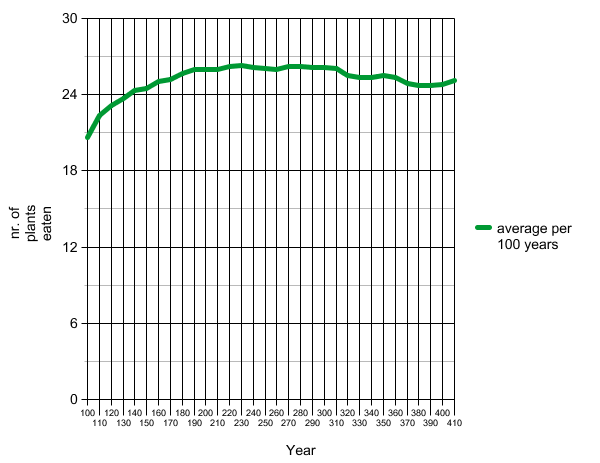
\includegraphics[width=10cm]{graph.png}\\
Crossover probability plays an important role in evolution, from the simulations we notice a difference between
between evolutions. The lower is the crossover probability, the worse an eater is evolving. This we can see on
the second graph, which represents the average plants eaten by an eater in 5 one hudred years average.\\
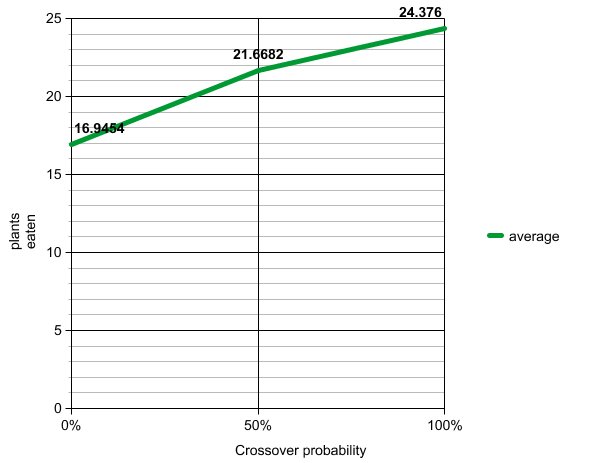
\includegraphics[width=10cm]{graph4.png}\\

\section*{Exercise 5}


\end{document}
